\documentclass[notheorems,9pt]{beamer}

% Packages with options
\usepackage[english]{babel}
\usepackage[mathscr]{euscript}
\usepackage[utf8]{inputenc}

% Primary Packages
\usepackage{amsbsy, amsmath, amssymb, amsthm, bm, commath, chngcntr, dsfont, econometrics, gensymb, graphicx, IEEEtrantools, longtable, marginnote, mathrsfs, mathtools, mdframed, natbib, parskip, pgf, setspace, subfigure, tabularx, textcomp, tikz, tkz-euclide,xcolor}

% Rest of the setup is in the "setup_beamer" package
\usepackage{setup_beamer}

% Title, Author, Institute
\title{Econ 103: Introduction}
\author{Manu Navjeevan}
\date{Summer Quarter, 2021}
\institute{UCLA}

%%%%%%%%%%%%%%%%%%%%%%%%%%%%%%%%%%%%%%%%%%%%%

\begin{document}
\frame{\titlepage}

\begin{frame}{Why Econometrics?} 
	Up till now, we have analyzed economic behavior by looking at economic theory.
	\begin{itemize}
		\item<1-> \ucla{Question:} Why do people go to the gym? \\ \ucla{Theory:} The benefit of joining the gym is higher than the cost. \\ \onslide<4->{\red{Data:} Many people sign up at the beginning of the year and stop going.}
		\item<2-> \ucla{Question:} What happens if we raise the minimum wage? \\ \ucla{Theory:} Unemployment will increase. \\ \onslide<5->{\red{Data:} At least for small increases, seems to be no effect.} 
		\item<3-> \ucla{Question:} Does it matter if we let people opt in or opt out? \\ \ucla{Theory:} Will not affect people's choices \\ \onslide<6->{\red{Data:} Opt out typically leads to higher uptake.}
	\end{itemize}	
\end{frame}

\begin{frame}{Why Econometrics?} 
	\begin{itemize}
		\item Economic Theory and modeling can teach us how to formally think through problems.
		\item Econometrics can help us fit parameters of our models or let us know if our models are correct.
	\end{itemize}
\end{frame}
\begin{frame}{Why Econometrics?} 
	Consider the simple supply and demand pricing model from Econ 1:
	\begin{figure}[htpb]
		\centering
		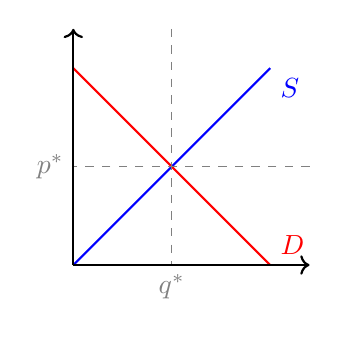
\begin{tikzpicture}
			\draw[blue,thick] (0,0)-- (2.5,2.5) node[anchor = north west] {\(S\)};
			\draw[red, thick] (0,2.5) -- (2.5,0) node[anchor = south west]{\(D\)};
			\draw[gray, dashed] (1.25,3)--(1.25,0) node[anchor = north] {\(q^*\)};
			\draw[gray, dashed] (3,1.25)--(0,1.25) node[anchor=east] {\(p^*\)};
			\draw[black, thick, ->] (0,0)--(0,3);
			\draw[black, thick, ->] (0,0)--(3,0);
		\end{tikzpicture}
		\caption{Equilibrium price and quantity}%
	\end{figure}
	\begin{itemize}
		\item<1-3|only@1-3>\ucla{Economic Theory:} Consumers maximize utility, producers maximize profit
		\begin{itemize}
			\item<2|only@2> Downward sloping demand and upward sloping supply
			\item<3|only@3> Theory can't tell us more about the curves exact shapes
		\end{itemize}
		\item<4-6|only@4-6>\ucla{Econometrics:} Estimate the supply/demand curve from data
		\begin{itemize}
			\item<5|only@5> Can reject theory if demand slopes upward
			\item<6|only@6> Theory can inform estimation technique
		\end{itemize}
	\end{itemize}
\end{frame}
\begin{frame}[t]{Why Econometrics?}
	\begin{minipage}[t][0.5\textheight]{\textwidth}
	\ucla{\bf Challenges in Econometrics:}
	\begin{itemize}
		\item<1-> Often in Econometrics we are interested in the \red{causal} relationship between two variables.
		\begin{itemize}
			\item<2-3|only@2-3> A demand curve is a causal relationship: what is the quantity demanded if the firm exogenously sets the price at  certain level?
			\item<3|only@3> May be interested in the effect of a certain policy: what would happen if we raised the minimum wage?
		\end{itemize}
		\item<4-> However, it is rare that we are able to run an experiment. 
		\begin{itemize}
			\item<5-6|only@5-6> As a third party researcher, cannot ask companies to randomly set some prices so that we can observe demand curve
			\item<6|only@6> Politically impractical (and potentially unethical!) to randomly implement a policy or assign people to treatment
		\end{itemize}
		\item<7-> Moreover, we often do not have a lot of data to work with when making our analyses
		\begin{itemize}
			\item<8-9|only@8-9> If we want to examine the effect of minimum wage increases typically look at a few cities that have implemented the policy
			\item<9|only@9> If we want to predict US GDP, only have about 150 years of economic data to use
		\end{itemize}
	\end{itemize}
	\end{minipage}
	\vfill
	\begin{center}
	{\ucla{\centering Have to think carefully about our econometric models and the inferences we draw from them.}}
	\end{center}
\end{frame}
\begin{frame}[fragile]{What will this course cover?} 
	This course will mainly focus on linear regression, a simple but powerful statistical model. 
	\begin{itemize}
		\item<1-> In some sense linear regression is easy.
		\begin{itemize}
			\item<1-> Plug and chug using \verb|R| or \verb|Python|.
			\item<1-> Lots of packages that will implement anything you want to do
		\end{itemize}
		\item<2-> However, doing linear regression \red{well} is hard.
		\begin{itemize}
			\item<2-> Correctly setting up models and figuring out how to interpret them requires careful thinking
			\item<2-> Oftentimes the ``easy'' interpretation can be very wrong
		\end{itemize}
	\end{itemize}
	\onslide<3->{In this course we will learn how to implement linear regression as well as how to correctly interpret the results from our regressions.}
\end{frame}
\begin{frame}{What will this course cover?} 
	Let's look at some potentially problematic conclusions to draw from data.
	\begin{figure}[htpb]
		\centering
		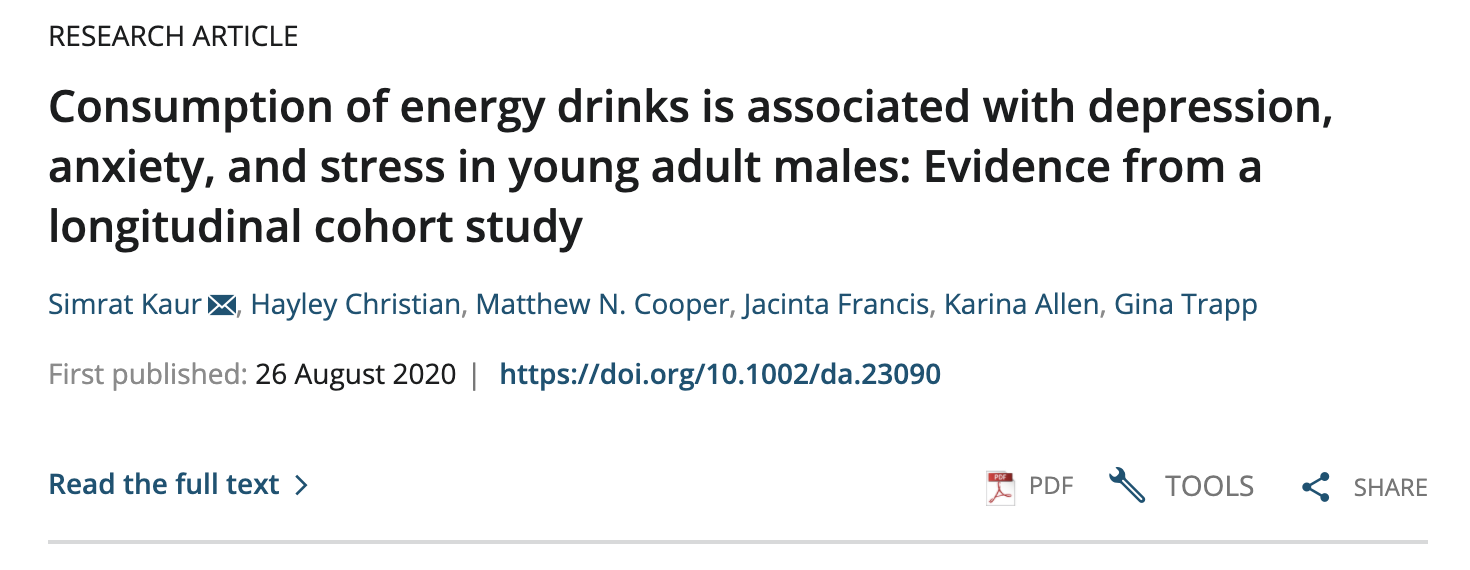
\includegraphics[width=0.8\linewidth]{energy_drinks.png}
		%\caption{}%
	\end{figure}
	\begin{itemize}
		\item At first read, easy to interpret paper as saying that consuming energy drinks leads to anxiety, depression, and stress
		\begin{itemize}
			\item But what types of people drink energy drinks?
			\item Are these people representative of the entire population?
			\item Can we definitively say that these people are stressed \emph{because} of the energy drinks? 
		\end{itemize}
	\end{itemize}
\end{frame}
\begin{frame}{What will this course cover?} 
	Let's look at some potentially problematic conclusions to draw from data.
	\begin{figure}[htpb]
		\centering
		
\includegraphics[width=0.8\linewidth]{greta.png}
	\end{figure}
	\begin{itemize}
		\item Paper found that people that attended a Greta Thunberg rally were more likely to engage in other forms of climate activism. 
		\begin{itemize}
			\item Is this causal?
			\item Perhaps! But people who are attending a Greta Thunberg rally may already be more likely to engage in other forms of climate activism.
		\end{itemize}
	\end{itemize}
\end{frame}
\begin{frame}{What will this course cover?} 
	Of course, predictive or associative analysis is still important.
	\begin{itemize}
		\item<1-> Can motivate further experimental/quasi-experimental research. 
		\item<2-> Can of interest by itself.
		\begin{itemize}
			\item In a medical settings, just want to use data to predict whether or not someone has cancer.
			\item Weathermen are (typically) just interested in forecasting the weather rather than the causal relationship between climate variables.
		\end{itemize}
	\end{itemize}
	\onslide<3->{Just have to be careful not predictive and causal analysis and precise about what exactly we can say from our statistical models.

	In this course we will not only focus on the mechanics of linear regression but also how to correctly interpret our results and use them to make careful inferences about the world.}
\end{frame}

\begin{frame}{What will this course cover?} 
	\begin{itemize}
		\item<1-> \red{Week 1: Econ 41 Review.} Single and multiple random variables; the normal distribution; law of large numbers and the central limit theorem; inference on the mean
		\item<2-> \red{Weeks 2-3: Single Linear Regression.} Linear regression with one explanatory variable; parameters of interest and their estimators; prediction and goodness of fit.
		\item<3-> \red{Weeks 4-5: Multiple Linear Regression.} Linear regression with more than one explanatory variable; modeling decisions; joint hypothesis testing; dummy variables.
		\item<4-> \red{Week 6: Beyond Linear Regression.} Causal inference; differences in differences; potential outcomes framework, non-linear models.
	\end{itemize}	
\end{frame}

\begin{frame}{Course Details} 
	\ucla{Pre-requisites}
	\begin{itemize}
		\item Econ 11 (Micro Theory) and Econ 41 (Statistics for Economists) or departmental approved equivalents
		\item Mainly will rely on material from Econ 41
	\end{itemize}
	\ucla{Co-requisite}
	\begin{itemize}
		\item Must also enroll in Econ 103L (lab section)
		\item Will mainly focus on coding in R, holding extra OH, and potentially covering 103 material if we fall behind
	\end{itemize}
\end{frame}

\begin{frame}{Course Detials} 
	\ucla{Remote Teaching}
	\begin{itemize}
		\item \red{Lecture Logistics.}
		\begin{itemize}
			\item Lectures and Lab Lectures will be held live at the alloted PST Time
			\begin{itemize}
				\item This allows for more interaction between me and you as well as among yourselves
			\end{itemize}
			\item Lectures will also be recorded and posted online to the CCLE page.
		\end{itemize}
	\item \red{Office Hours.}
	\begin{itemize}
		\item My office hours will be held Tuesdays at 11am-12pm and again at 9pm-10pm PST
		\item TA will post their own office hours
		\item Happy to stay after lecture and answer questions as well
	\end{itemize}
	\end{itemize}
\end{frame}

\begin{frame}[t]{Course Details} 
	\ucla{Contact Information}
	\begin{itemize}
		\item For questions outside of office hours, can reach out to me at \ucla{mnavjeevan@g.ucla.edu}
		\item Can also open up a discussion on the CCLE page 
		\begin{itemize}
			\item This way everyone can see your question and you may be able to get help from other students
		\end{itemize}
		\only<1>{
		\begin{figure}[htpb]
			\centering
			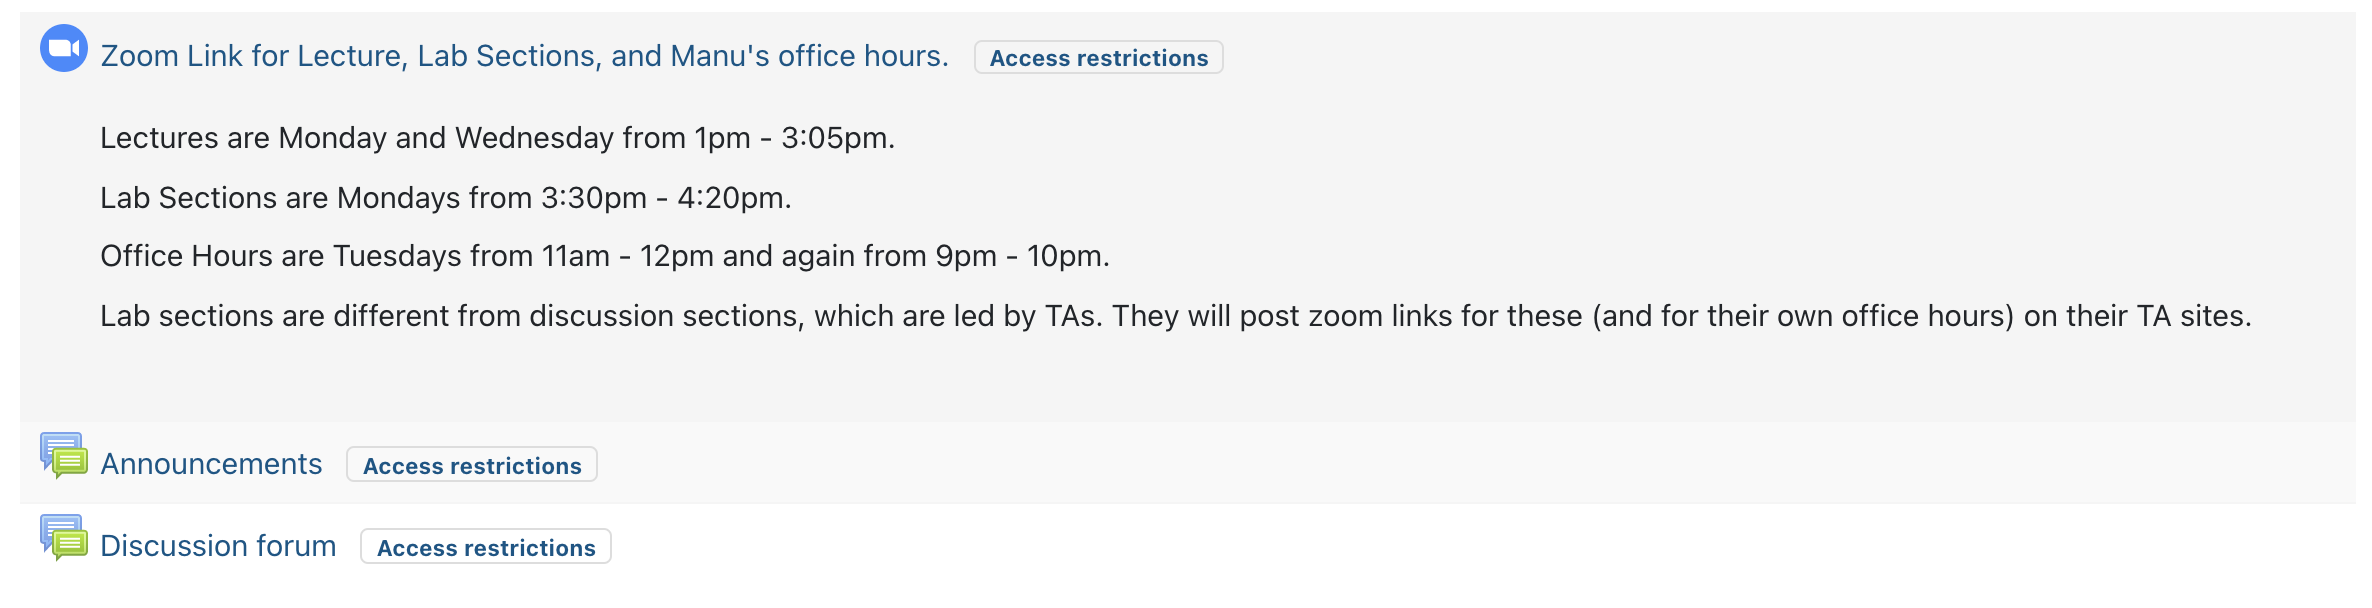
\includegraphics[width=0.95\linewidth]{CCLE.png}
	\end{figure}}
	\only<2->{
	\begin{figure}[htpb]
		\centering
		
\includegraphics[width=0.95\linewidth]{discussion.png}
	\end{figure}}
	\end{itemize}
\end{frame}

\begin{frame}{Course Details} 
	\ucla{Grading}
	\begin{itemize}
		\item<1-> \red{Problem Sets (60\% of final grade)}
		\begin{itemize}
			\item Half credit for completion, other half for correctness
			\item Mix of theory and R coding
			\item Must be handed in on time via CCLE
			\item Problem Sets will be assigned at the beginning of weeks 2, 3,and 5 and will be due at the beginning of weeks 3, 4, and 6.
		\end{itemize}
		\item<2-> \red{Midterm (20\% of final grade)}
		\begin{itemize}
			\item Administered Wednesday of week 4 via CCLE, covering up to single linear regression.
			\item Will be given a 24 hour period in which to complete the exam, which should not take more than an hour and a half.
		\end{itemize}
		\item<3-> \red{Final Project (20\% of final grade)}
		\begin{itemize}
			\item Data exercise, will be given a data set and ask them to come up with an appropriate statistical model
		\end{itemize}
	\end{itemize}
\end{frame}

\begin{frame}{Questions?} 
	\centering\red{Questions?} 
\end{frame}

\end{document}


